%\documentclass{article}
\documentclass[12pt,a4paper]{report}
\usepackage{amsmath,epsfig,rotating}
\usepackage{subcaption} % For aligning subfigures
\usepackage{pdfpages}

\usepackage[utf8]{inputenc} % For Unicode characters
\usepackage{graphicx} % For including images
\usepackage{amsmath,amssymb} % For mathematical symbols
%\usepackage{hyperref} % For clickable links in PDF
\usepackage{geometry} % To adjust margins
\usepackage{float}
\usepackage{titlesec}
\usepackage[hidelinks]{hyperref}
\hyphenpenalty=1000 % Allow some hyphenation to prevent overfull boxes
\usepackage{xcolor}
\hypersetup{
    colorlinks=true,
    linkcolor=black,
    citecolor=black,
    filecolor=black,
    urlcolor=black
}


%\geometry{showframe}
\titleformat{\chapter}[display]
  {\normalfont\centering\large\bfseries}
  {\makebox[0pt][c]{\chaptername\ \thechapter}}{6pt}{\large\vspace*{8pt}}


%\geometry{margin=1in} % Set 1-inch margins
\geometry{
  left=1.5in,    % Left margin
  right=1in,     % Right margin
  top=1in,       % Top margin
  bottom=1in     % Bottom margin
}
% Title page information
%\title{}
%\author{}
%\date{}
\renewcommand{\bibname}{References} % For article class

\begin{document}


\includepdf[pages={1}]{CoverPage.pdf}  % Include pages 1 to 3


\tableofcontents
\newpage


\begin{abstract}
Quantum Legacy is a cutting-edge sci-fi tower defense game that immerses players in a futuristic universe where strategic planning and quick decision-making are key to survival. Featuring 8 unique towers, each with distinct abilities and upgrade paths, players must defend their base against waves of alien invaders across 4 meticulously designed levels, each offering unique terrain and environmental challenges. The game includes a Towers Shop for strategic tower selection, a Settings Menu for customizable sound and graphics, a robust Saving System to track currency and experience, and a Username Change System for personalization. With its blend of tactical gameplay, immersive visuals, and a rewarding progression system, Quantum Legacy delivers an engaging and dynamic experience for both casual and hardcore gamers. Designed for PC and mobile, the game sets the stage for future expansions, including multiplayer modes and additional content, ensuring long-term replayability and growth.
\end{abstract}

%\newpage

\chapter{Introduction}
%\section{Introduction}
Quantum Legacy is a fast-paced, strategic tower defense game set in a futuristic sci-fi universe. Players must defend their base from waves of alien invaders by strategically placing and upgrading towers. With a blend of tactical gameplay, immersive visuals, and a progression system, the game offers a rewarding experience for both casual and hardcore gamers.  

\section{Background}
Tower defense (TD) games are a strategy subgenre where players defend a base by placing and upgrading towers to stop waves of enemies. Core mechanics include tower variety, enemy waves, resource management, and strategic level design. Popular themes range from fantasy and sci-fi to historical settings, appealing to a wide audience. TD games are known for their accessibility, replayability, and strategic depth, making them a staple on PC, consoles, and mobile devices. Originating as custom maps in games like Warcraft III, the genre has evolved with modern titles like Kingdom Rush and Bloons TD 6, incorporating advanced graphics, RPG elements, and multiplayer modes. The future of TD games may include VR/AR integration, cross-platform play, and procedural generation, ensuring the genre remains dynamic and engaging.

\section{Unity Game Engine}
The Unity Game Engine is a powerful and versatile game development platform used for creating 2D, 3D, AR, and VR experiences across multiple platforms, including PC, consoles, mobile devices, and web browsers. Known for its user-friendly interface, real-time rendering, and extensive asset store, Unity enables developers of all skill levels to build games efficiently. Unity is built around a component-based architecture, where objects in a scene, known as GameObjects, can be customized using scripts, physics, animations, and UI elements. It supports C\# scripting, allowing developers to write custom game logic using the MonoBehaviour system. The engine also includes powerful tools such as NavMesh for AI pathfinding, Cinemachine for camera control, and Unity Physics for realistic interactions. One of Unity’s greatest strengths is its cross-platform support, enabling developers to build once and deploy to multiple platforms with minimal adjustments. Additionally, Unity offers a robust Asset Store, where developers can access a vast library of ready-to-use assets, scripts, and plugins. Unity is widely used across the game industry for both indie and AAA game development, as well as in fields like simulation, architecture, film production, and machine learning. Its continuous updates and growing community make it a top choice for game developers worldwide.

\section{Unity Tower Defense Template}
The Unity Tower Defense Template provides a structured framework for developing a tower defense game using Unity. It includes essential features such as main menu navigation, level selection, tower placement, enemy waves, and game progression mechanics. This template allows developers to quickly set up a game where players can select levels, build defensive structures, and defend against incoming enemies.

%In the main menu, players can access options like Settings. The level selection system enables players to choose different stages, with the possibility of unlocking new levels based on progress. During gameplay, players strategically place towers on a predefined map to attack and eliminate enemy units. The system includes mechanics for enemy AI movement, tower targeting logic, wave spawning, and health management.

The template follows a modular design, allowing easy customization of tower attributes, enemy behaviors, and difficulty scaling. It integrates UI elements, animations, and sound effects to enhance user experience. Upon completing a level, players can either return to the main menu or continue playing, ensuring a seamless game loop.

This template serves as a solid foundation for developing a full-fledged tower defense game, offering flexibility for further enhancements such as upgradable towers, special abilities, and multiplayer features. 

The Tower defense Template is made using two reusable frameworks.
\subsection{Action Game Framework}
The first framework is called the Action Game Framework. The Action Game Framework
includes code that covers concepts needed in action games, such as taking damage and logic
for ballistics and projectiles.

\subsection{Core Framework}
The second framework is called the Core Framework. The Core Framework covers concepts
that are common to games of all genres, such as game saving, data management, timers, math
utilities and more

\begin{figure}[h!]
	\centering
	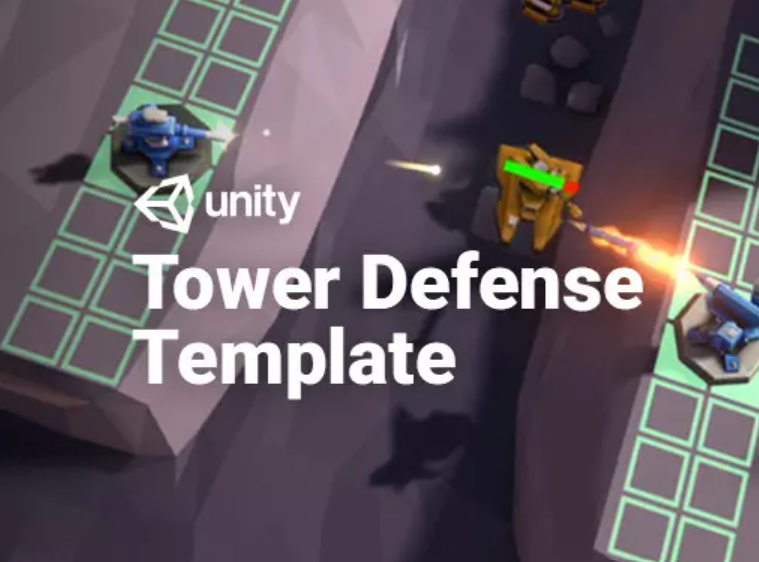
\includegraphics[scale=0.5]{images/UnityTDTemplate.png}
	\caption{Unity Tower Defense Template}
	\label{fig:UnityTDTemplate}
\end{figure}


\chapter{Methodology}
In this chapter, we describe the methods for extending the Unity Tower Defense template to make it a fully functional tower defense game instead of a prototype. Section \ref{sec:GameFlow} describes the main game flow while other sections describe the additional features of our project.

\section{Game Flow}
\label{sec:GameFlow}
\begin{figure}[h!]
	\centering
	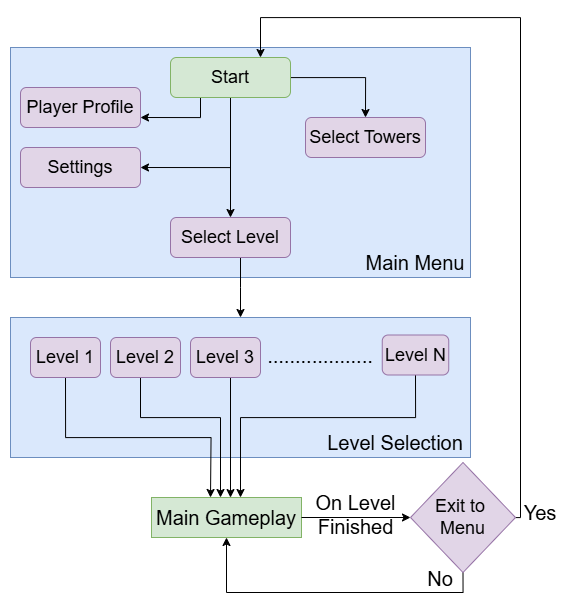
\includegraphics[scale=0.55]{images/GDLabProjFlowChart.png}
	\caption{Gameplay Flowchart}
	\label{fig:GameplayFlowchart}
\end{figure}

Figure \ref{fig:GameplayFlowchart} outlines the user navigation flow in this game, detailing the interactions between the main menu, level selection, and gameplay. The process begins at the Start node, where players can access different features such as Player Profile, Settings, and Select Towers Menu before proceeding to Select Level. The Level Selection section presents multiple levels, allowing players to choose one before transitioning into Main Gameplay. Once a level is completed, a decision point determines whether the player returns to the menu or continues playing

\section{Towers}
Players have access to 8 distinct towers, each with unique abilities, strengths, and upgrade paths. Examples include:  
\begin{itemize}
    \item \textbf{Machine Gun}: High damage, single-target attacks.  
    \item \textbf{EMP}: Slows nearby enemies down.
    \item \textbf{FlameThrower}:  Breathes Fire at enemies.
    \item \textbf{Laser}: Shoots laser beams with long range, high damage, slow fire rate. 
    \item \textbf{Mega Laser}: Better version of Laser Tower  
    \item \textbf{Mortar}: High AoE damage on ground enemies only. 
    \item \textbf{Missile Launcher}: Fires homing missiles for heavy damage.  
    \item \textbf{Energy Pylon}: Generates Energy 
\end{itemize}

Each tower can be upgraded up to 3 levels (during gameplay), enhancing its power, range, and special abilities.

\section{Levels}  
The game features 4 meticulously designed levels, each with its own terrain, enemy types, and challenges.  
Each level introduces new enemy types and environmental hazards, requiring players to adapt their strategies.

\section{Towers Shop and Selection}  
Before each level, players can visit the \textbf{Towers Shop} to purchase and select up to 4 towers for the upcoming battle. The shop features:  
\begin{itemize}
    \item \textbf{Tower Unlocks}: New towers can be unlocked using in-game currency earned from completing levels.  
    \item \textbf{Strategic Selection}: Choosing the right combination of towers is crucial for success. A player can select only 4 cards at a time.  
\end{itemize}

\section{Settings Menu}  
The game includes a comprehensive \textbf{Settings Menu} to customize the player’s experience:  
\begin{itemize}
    \item \textbf{Sound Settings}: Adjust master volume, music, and sound effects.  
    \item \textbf{Graphics Settings}: Toggle between low, medium, and high graphics presets.  
\end{itemize}

\section{Saving System}  
The game features a robust \textbf{Saving System} to track player progress. User data is encrypted in a file and saved in the persistant path of device:  
\begin{itemize}
    \item \textbf{Currency}: Earned by defeating enemies and completing levels. Used to purchase and upgrade towers.  
    \item \textbf{Experience Points (XP)}: Gained by completing levels and achieving objectives. Levels up the player profile, unlocking new towers and abilities.  
    \item \textbf{Auto-Save}: Progress is automatically saved after each level, ensuring no progress is lost.  
\end{itemize}

\section{Username Change System}  
Players can personalize their experience with a \textbf{Username Change System}:  
\begin{itemize}
    \item \textbf{Custom Username}: Players can set or change their in-game username at any time.  
    \item \textbf{Profile Integration}: Usernames are displayed on leaderboards and in multiplayer modes (if added in future updates).  
\end{itemize}

\chapter{Some Important Code Screenshots}
%
\includepdf[pages={1}]{CoverPage.pdf}  % Include pages 1 to 3

\section{TowerLibrary.cs} 
\begin{figure}[h!]
	\centering
	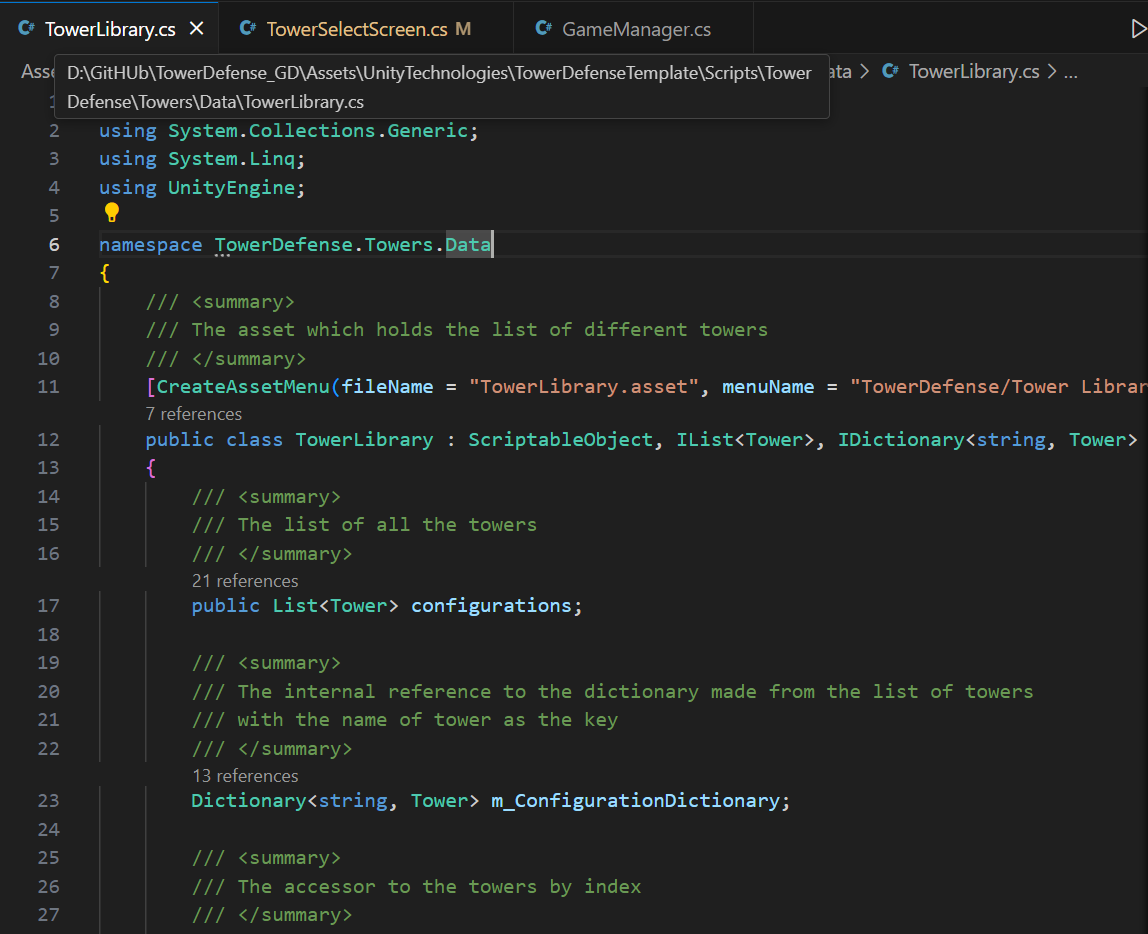
\includegraphics[scale=0.8]{images/TowerLibrary.png}
	\caption{TowerLibrary Script}
	\label{fig:TowerLibrary}
\end{figure}

The Script in Figure \ref{fig:TowerLibrary} is a ScriptableObject that manages a collection of Tower objects, providing both list-based and dictionary-based access. It implements IList and IDictionary to enable retrieval by index and by tower name.

\section{TowerLevelData.cs} 
\begin{figure}[h!]
	\centering
	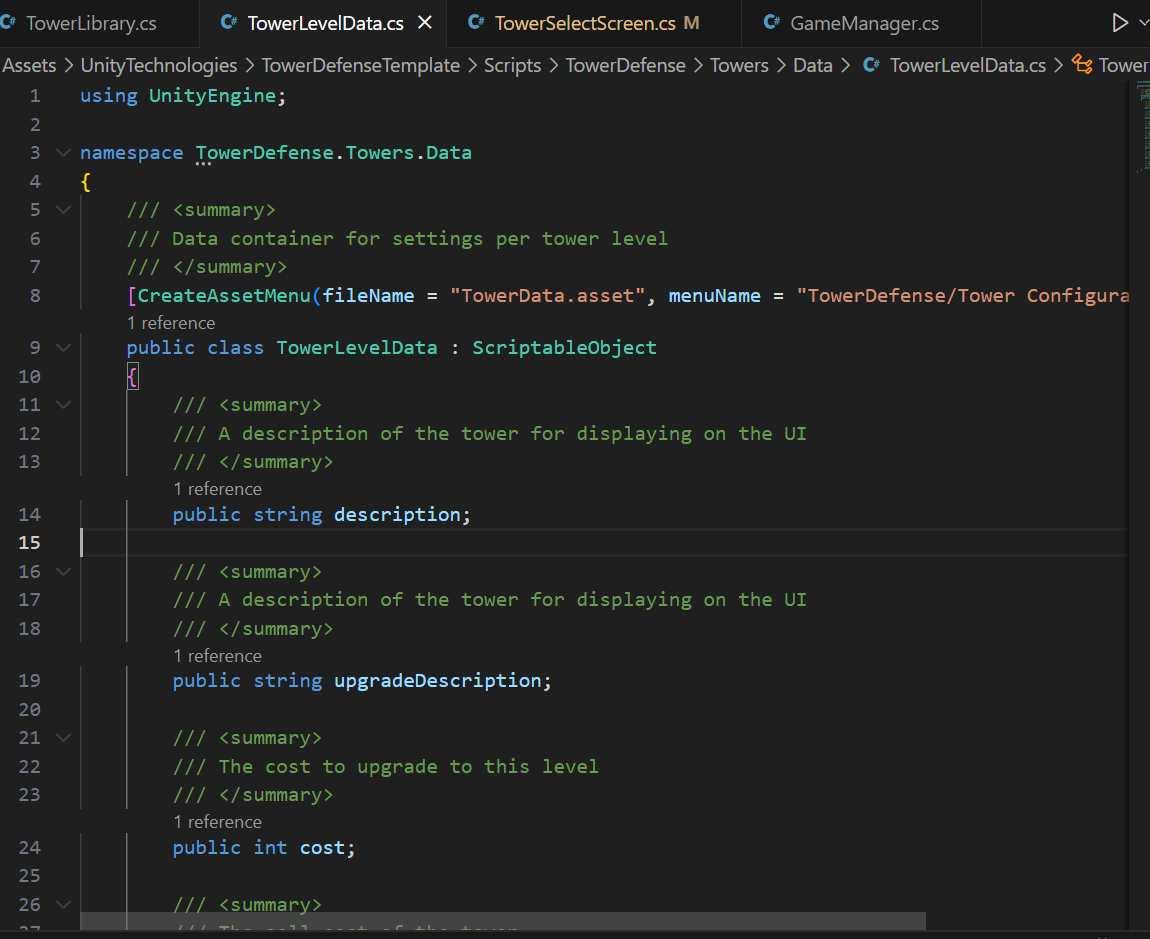
\includegraphics[scale=0.75]{images/TowerLevelData1.png}
	\caption{TowerLevelData Script Part 1}
	\label{fig:TowerLevelData1}
\end{figure}

\begin{figure}[h!]
	\centering
	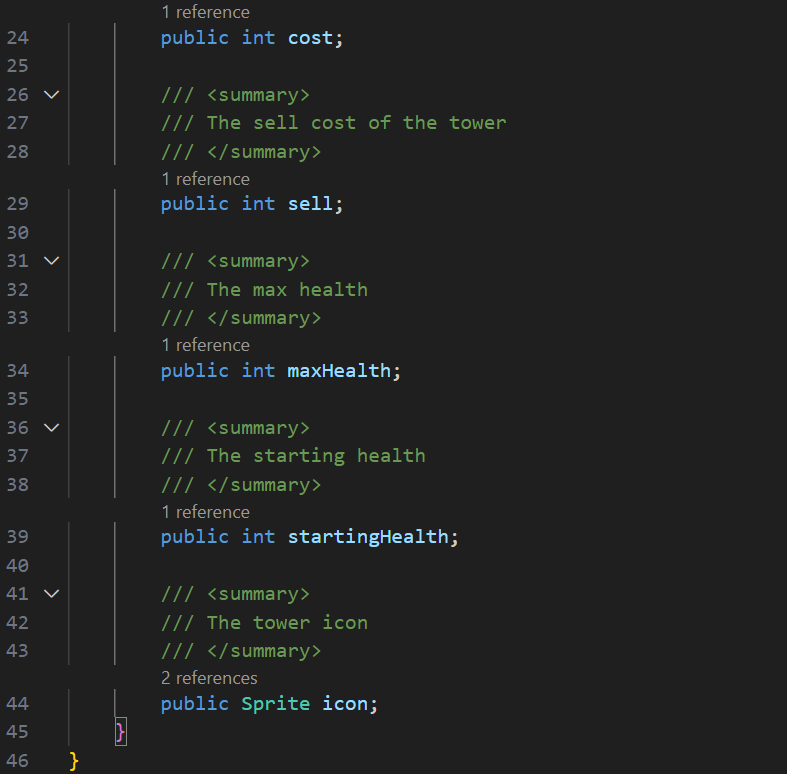
\includegraphics[scale=0.75]{images/TowerLevelData2.png}
	\caption{TowerLevelData Script Part 2}
	\label{fig:TowerLevelData2}
\end{figure}

The script in figure [\ref{fig:TowerLevelData1},\ref{fig:TowerLevelData2}] is a `ScriptableObject` that stores settings for each tower level, including descriptions, cost, health, and an icon for UI display. It helps manage tower upgrades and attributes in a Tower Defense game.


\section{GameManager.cs}

\begin{figure}[h!]
	\centering
	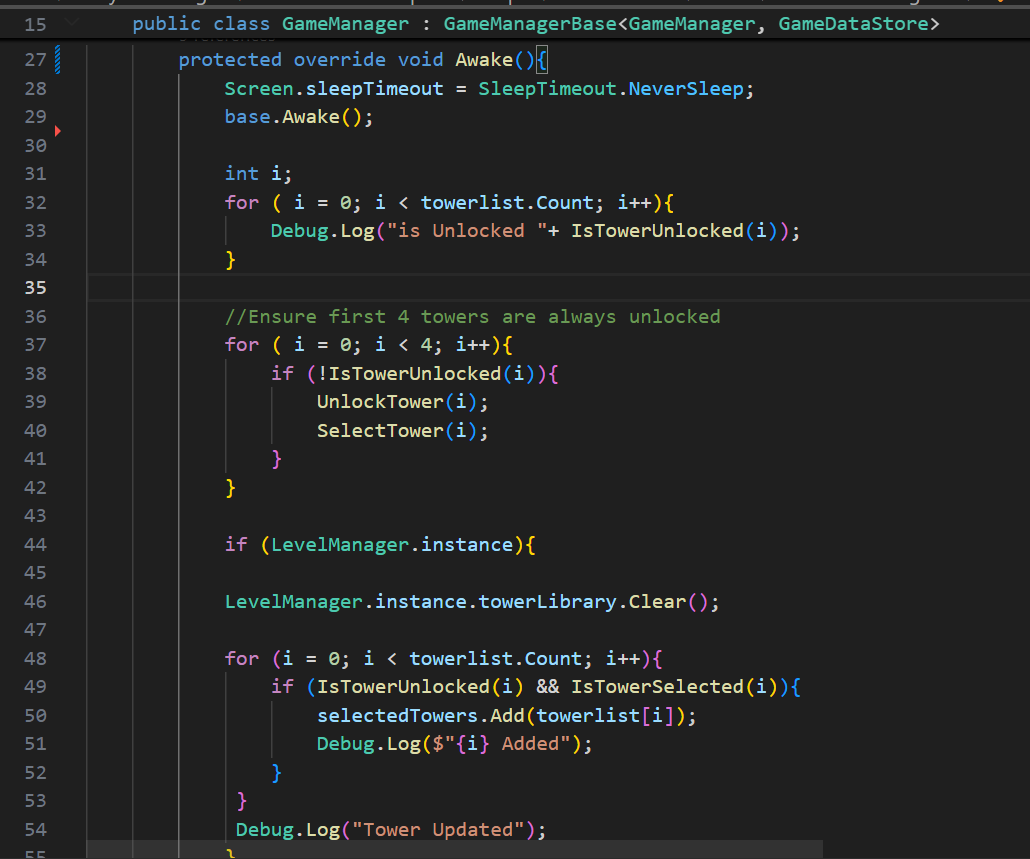
\includegraphics[scale=0.75]{images/GameManager1.png}
	\caption{GameManager Script Part 1}
	\label{fig:GameManager1}
\end{figure}

\begin{figure}[h!]
	\centering
	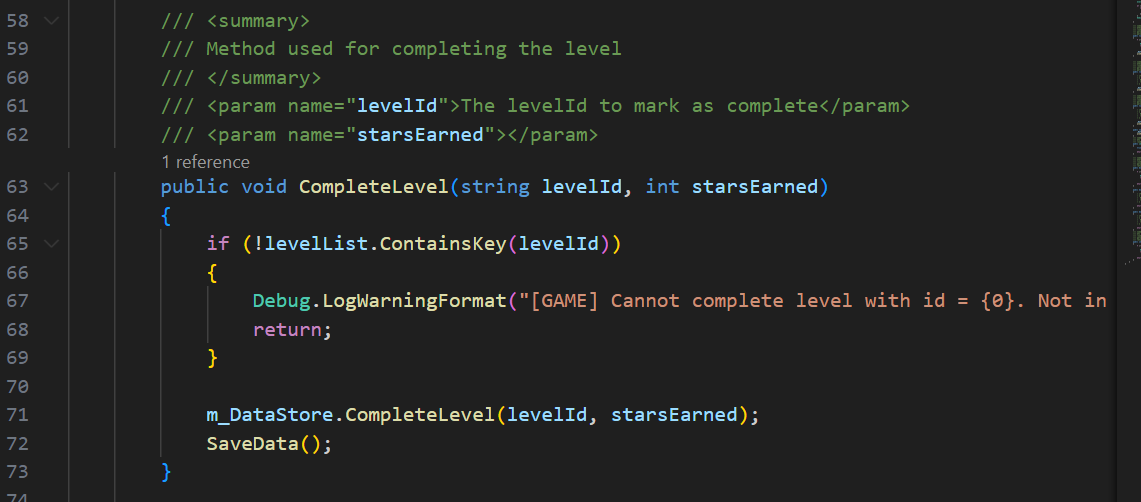
\includegraphics[scale=0.75]{images/GameManager2.png}
	\caption{GameManager Script Part 2}
	\label{fig:GameManager2}
\end{figure}

\begin{figure}[h!]
	\centering
	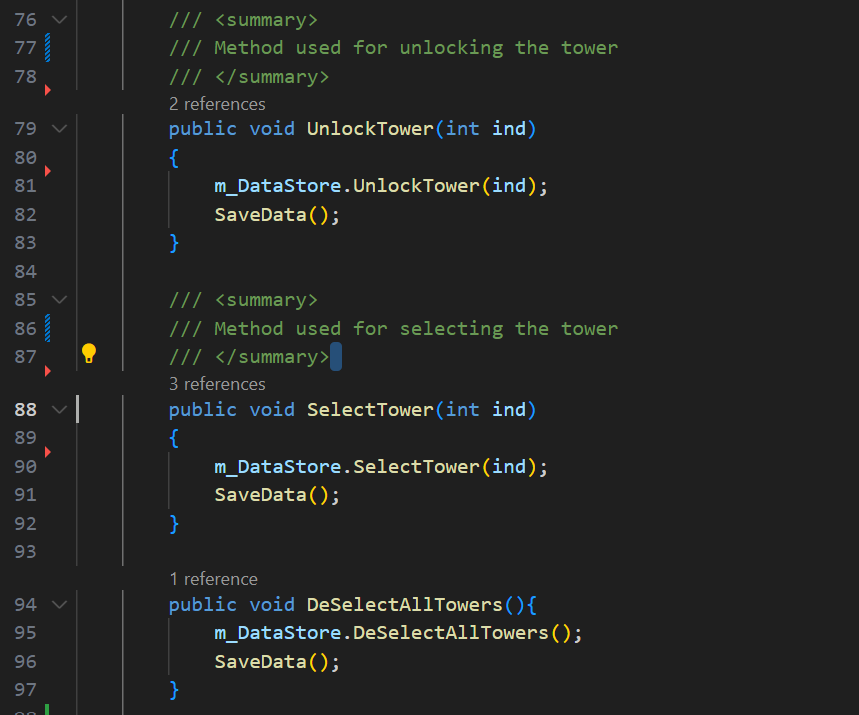
\includegraphics[scale=0.75]{images/GameManager3.png}
	\caption{GameManager Script Part 3}
	\label{fig:GameManager3}
\end{figure}

\begin{figure}[h!]
	\centering
	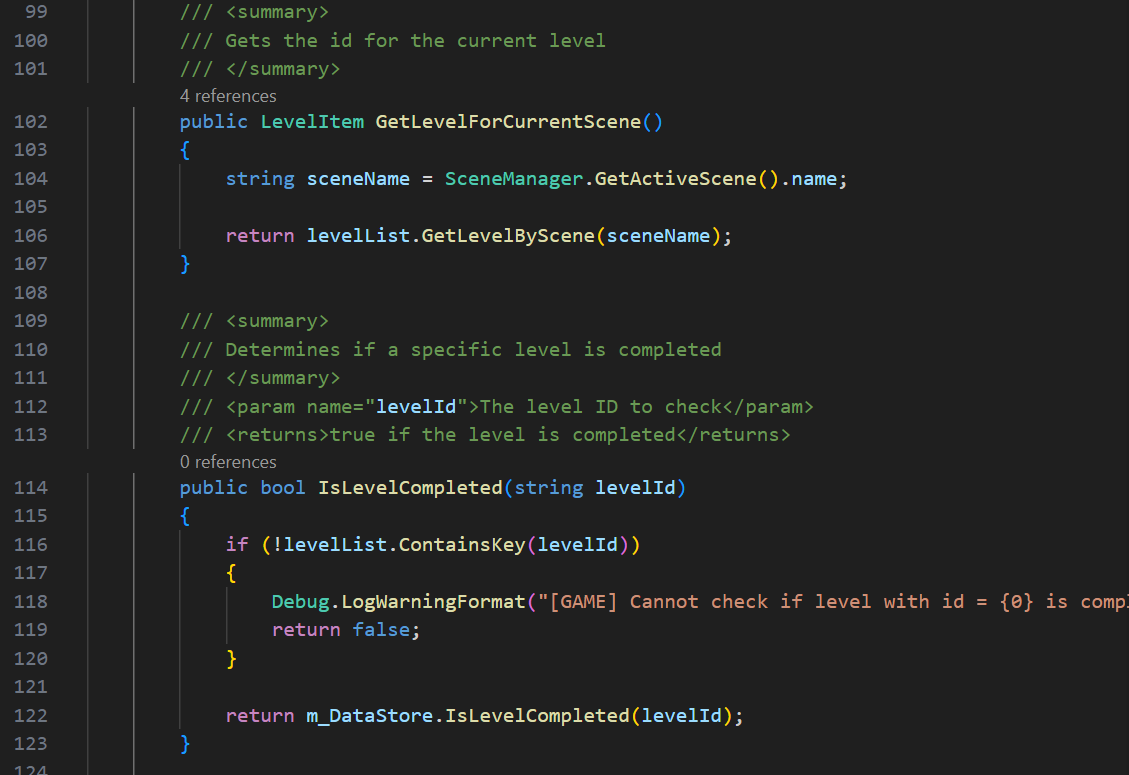
\includegraphics[scale=0.75]{images/GameManager4.png}
	\caption{GameManager Script Part 4}
	\label{fig:GameManager4}
\end{figure}

\begin{figure}[h!]
	\centering
	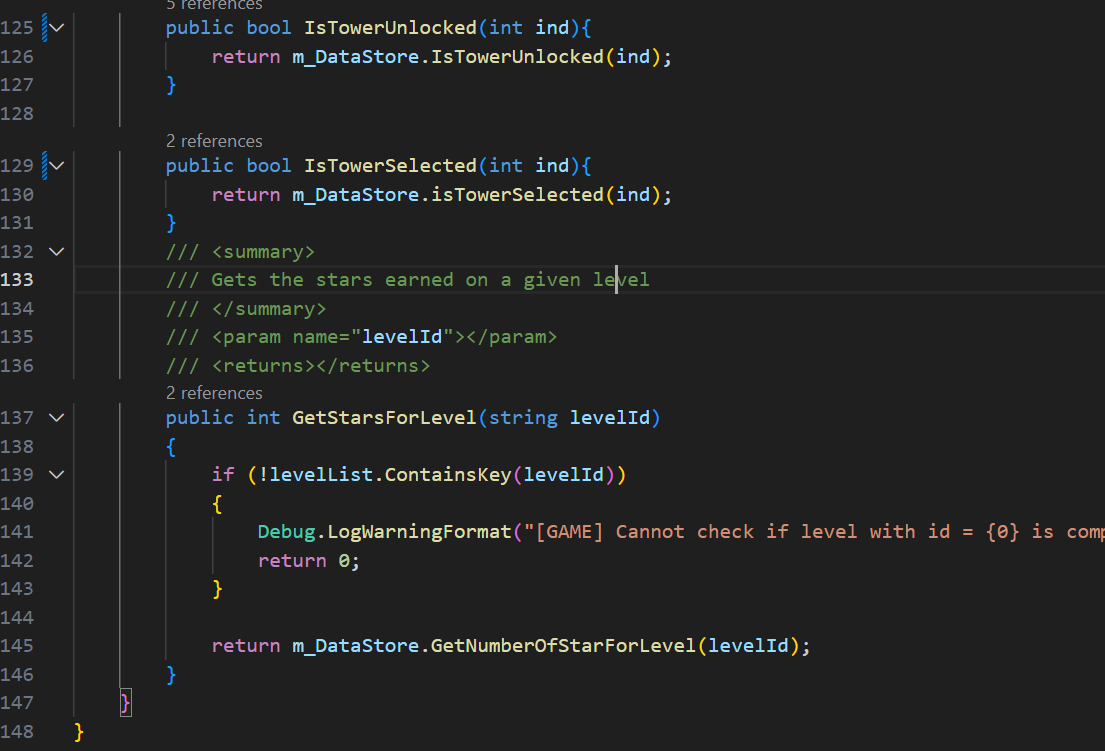
\includegraphics[scale=0.75]{images/GameManager5.png}
	\caption{GameManager Script Part 5}
	\label{fig:GameManager5}
\end{figure}

\section{GameDataStore.cs}
\begin{figure}[h!]
	\centering
	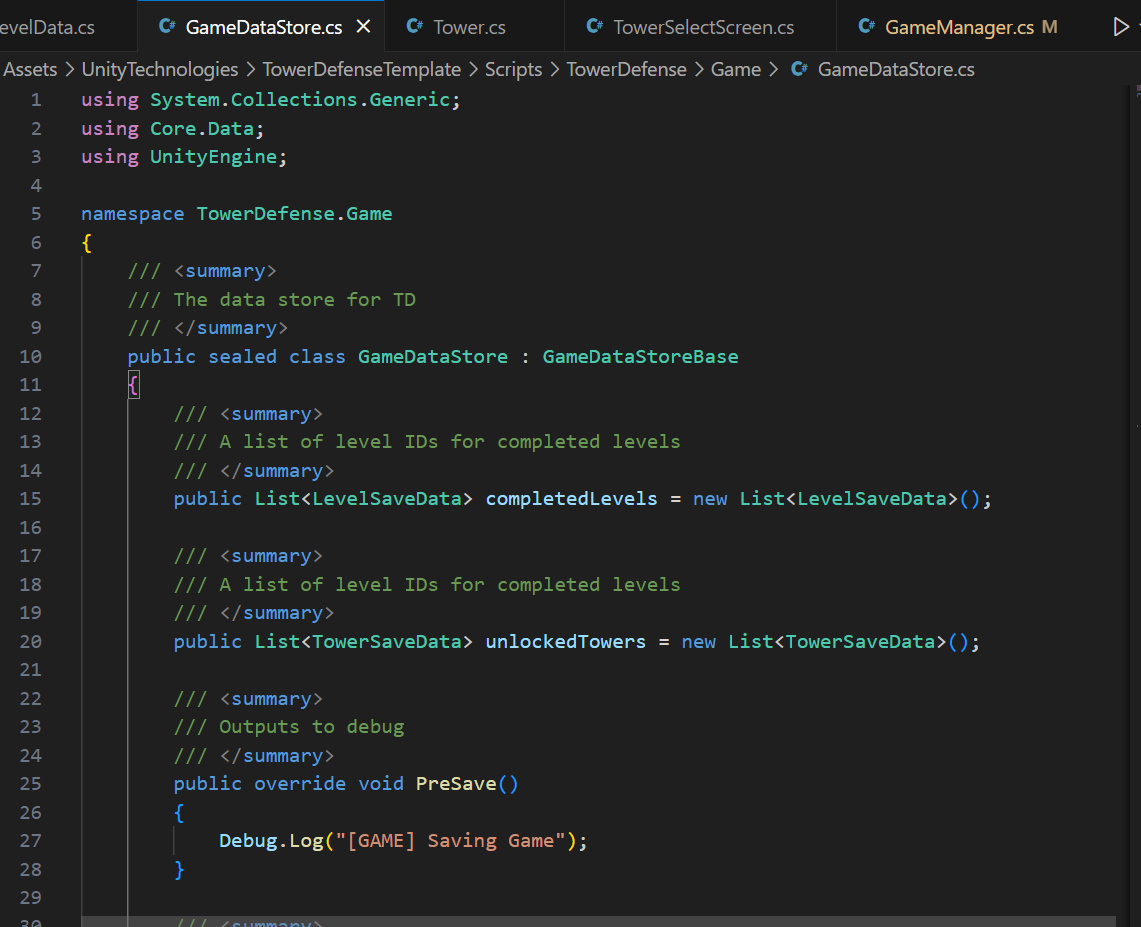
\includegraphics[scale=0.75]{images/GameDataStore1.png}
	\caption{GameDataStore Script Part 1}
	\label{fig:GameDataStore1}
\end{figure}
 
\begin{figure}[h!]
	\centering
	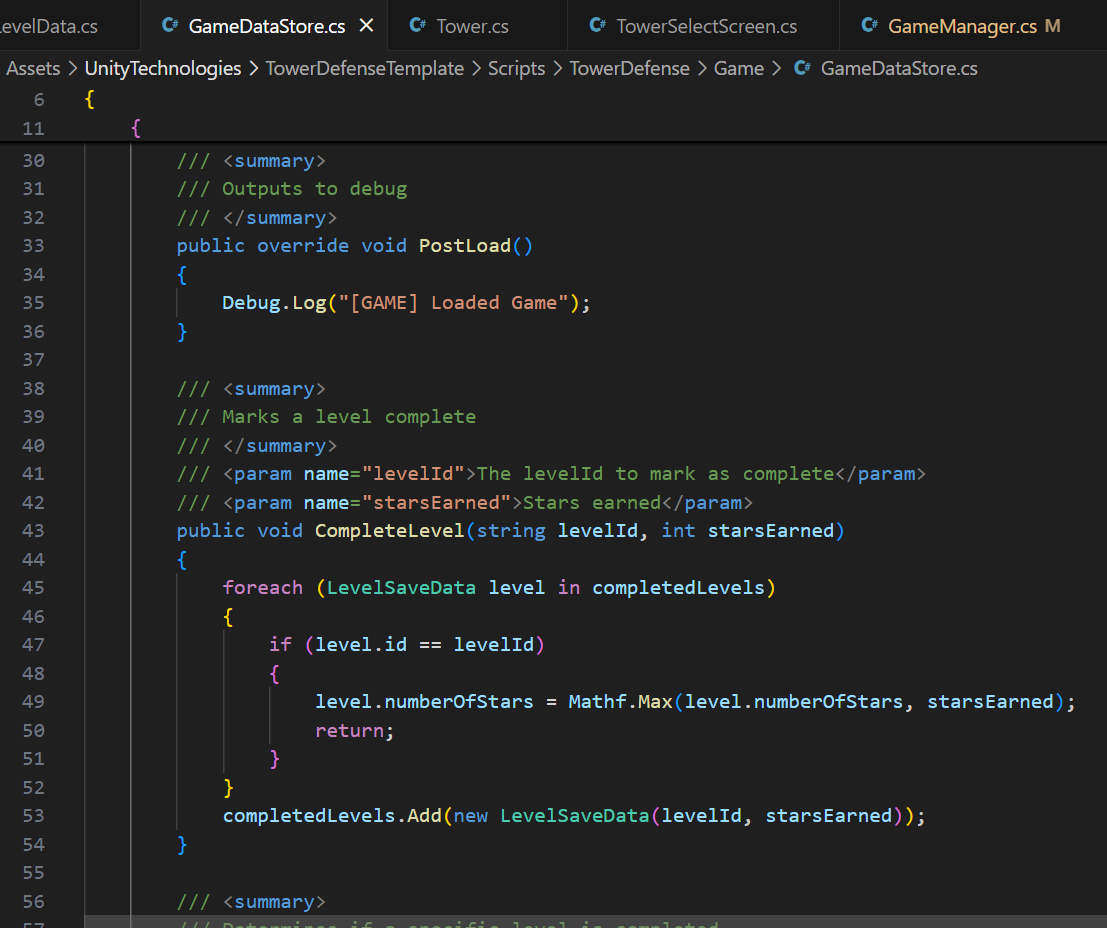
\includegraphics[scale=0.75]{images/GameDataStore2.png}
	\caption{GameDataStore Script Part 2}
	\label{fig:GameDataStore2}
\end{figure}
 
\begin{figure}[h!]
	\centering
	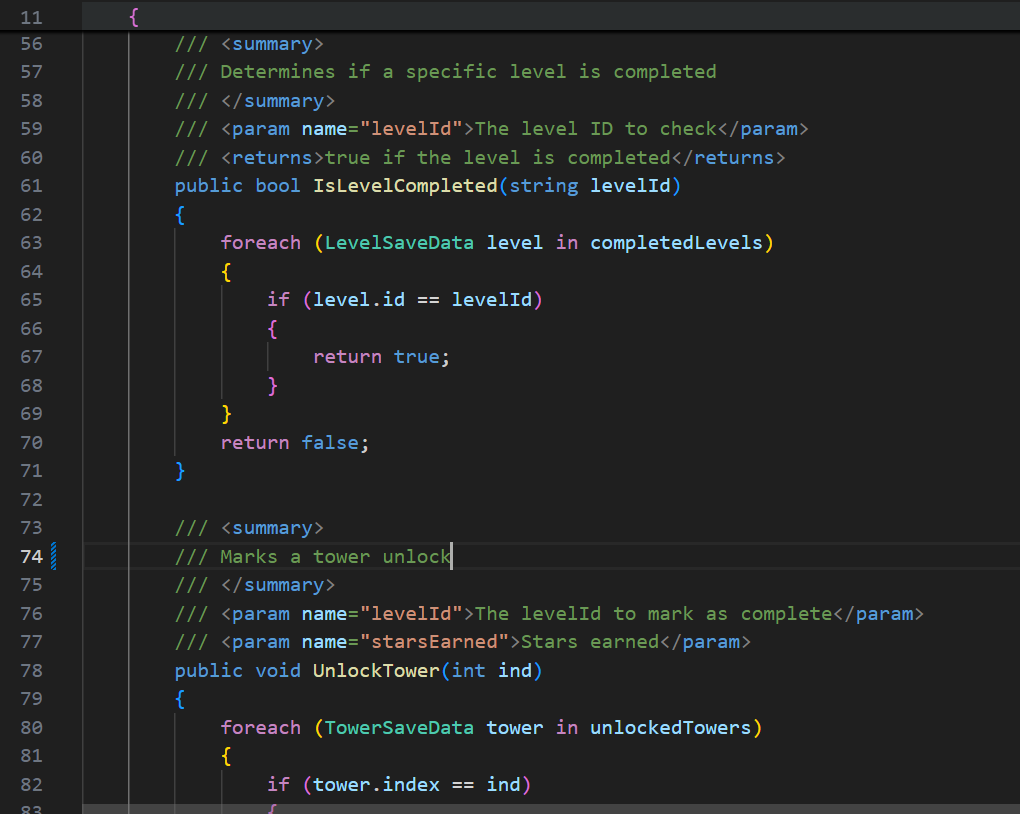
\includegraphics[scale=0.75]{images/GameDataStore3.png}
	\caption{GameDataStore Script Part 3}
	\label{fig:GameDataStore3}
\end{figure}
 
\begin{figure}[h!]
	\centering
	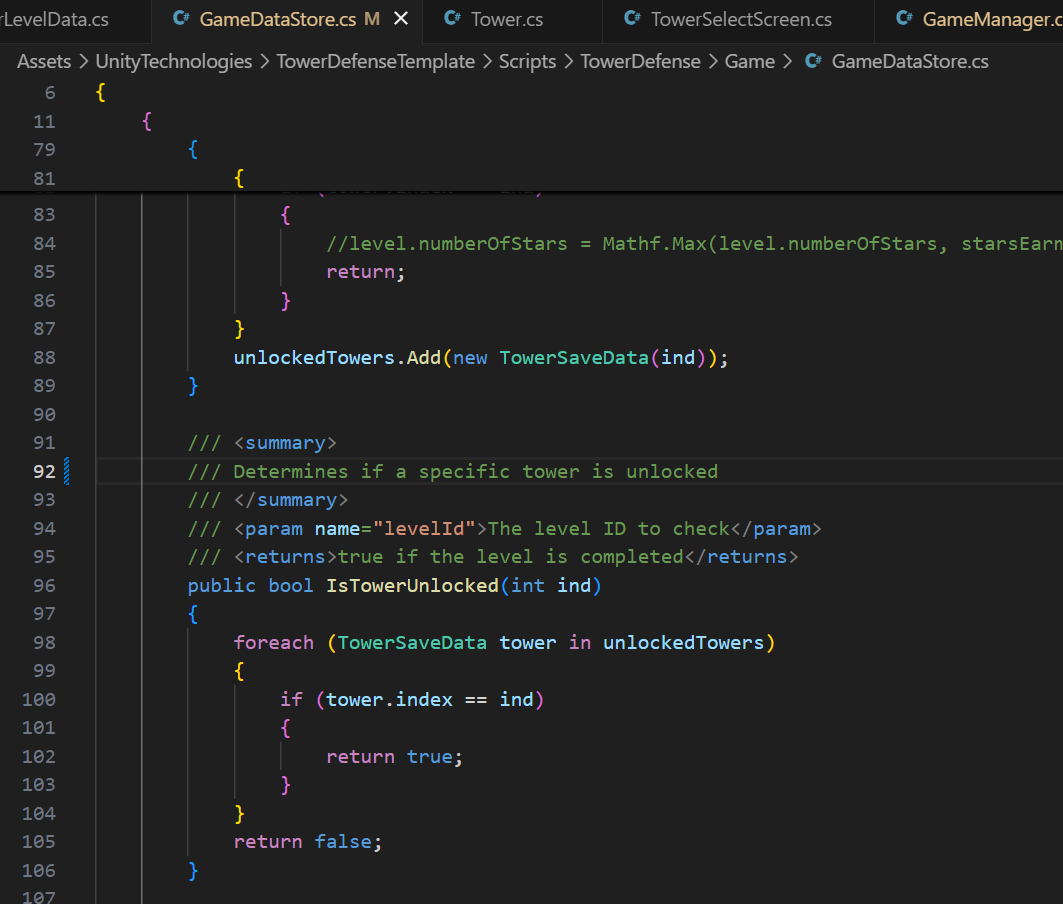
\includegraphics[scale=0.75]{images/GameDataStore4.png}
	\caption{GameDataStore Script Part 4}
	\label{fig:GameDataStore4}
\end{figure}
 
\begin{figure}[h!]
	\centering
	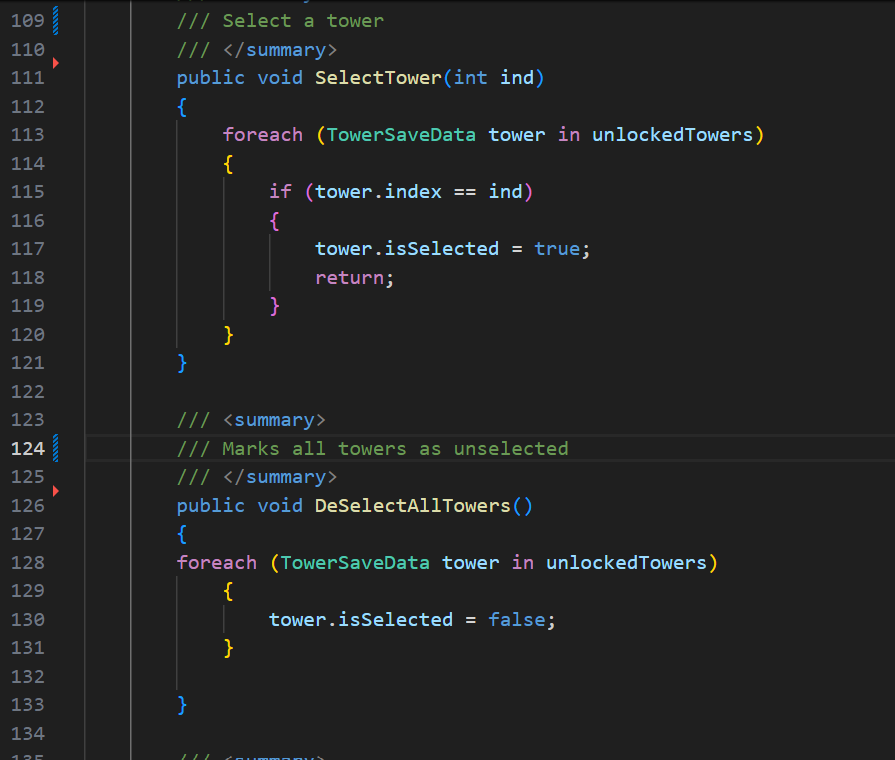
\includegraphics[scale=0.75]{images/GameDataStore5.png}
	\caption{GameDataStore Script Part 5}
	\label{fig:GameDataStore5}
\end{figure}
 
\begin{figure}[h!]
	\centering
	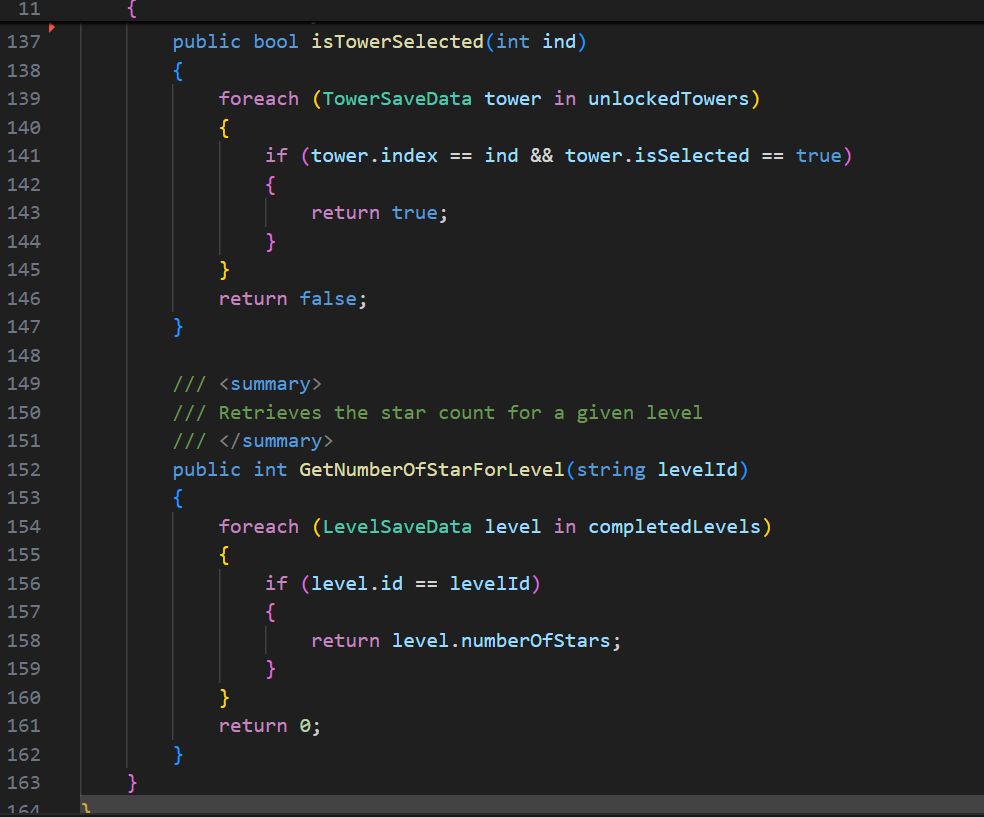
\includegraphics[scale=0.75]{images/GameDataStore6.png}
	\caption{GameDataStore Script Part 6}
	\label{fig:GameDataStore6}
\end{figure}
 
\section{LevelSaveData.cs}
 
\begin{figure}[h!]
	\centering
	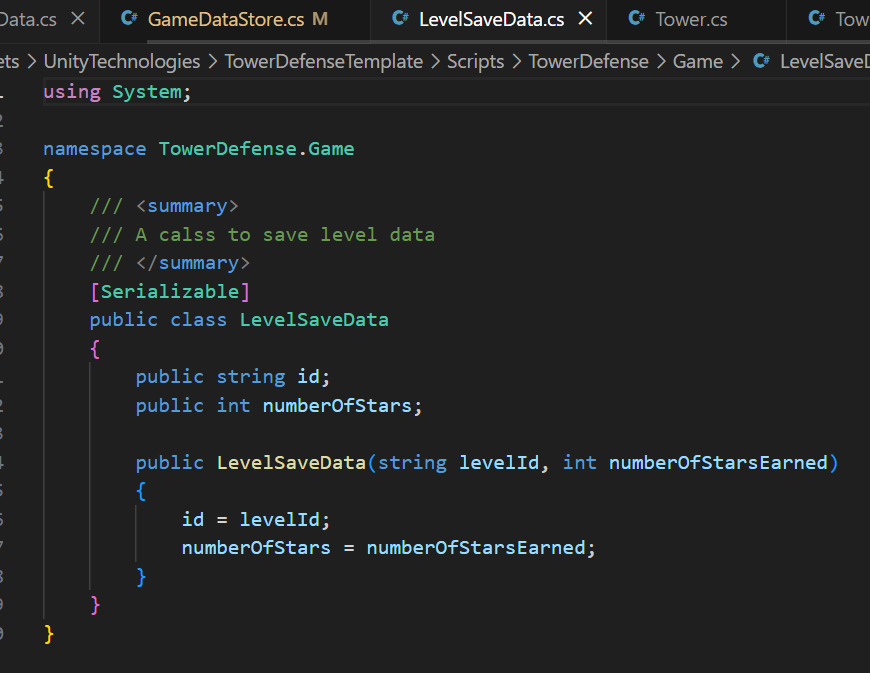
\includegraphics[scale=0.75]{images/LevelSaveData.png}
	\caption{LevelSaveData Script}
	\label{fig:LevelSaveData}
\end{figure}


\section{TowerSaveData.cs}
\begin{figure}[h!]
	\centering
	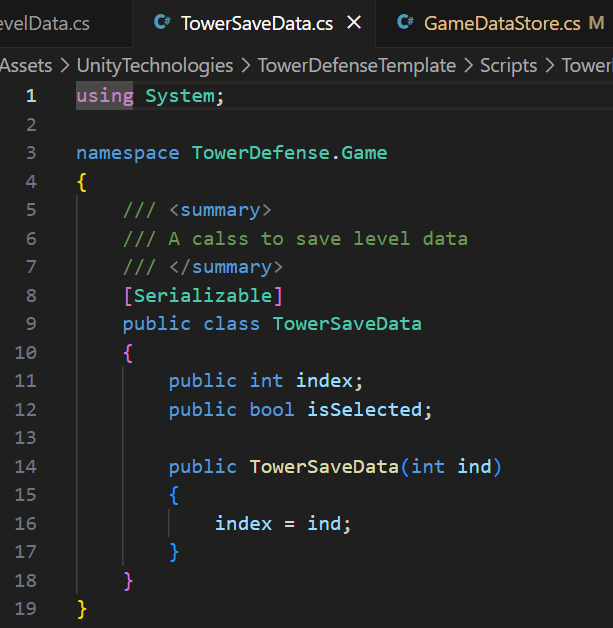
\includegraphics[scale=0.75]{images/TowerSaveData.png}
	\caption{TowerSaveData Script}
	\label{fig:TowerSaveData}
\end{figure}

\begin{figure}[h!]
	\centering
	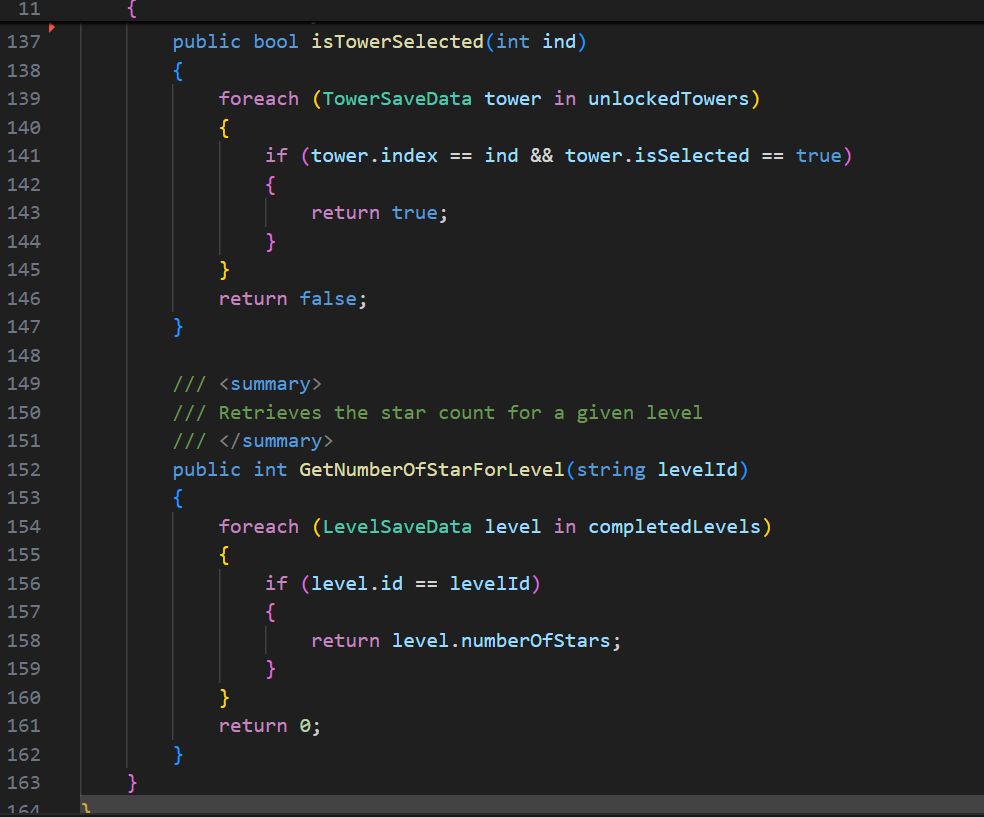
\includegraphics[scale=0.75]{images/GameDataStore6.png}
	\caption{GameDataStore Script Part 6}
	\label{fig:GameDataStore6}
\end{figure}

\section{CardDragHandler.cs}
\begin{figure}[h!]
	\centering
	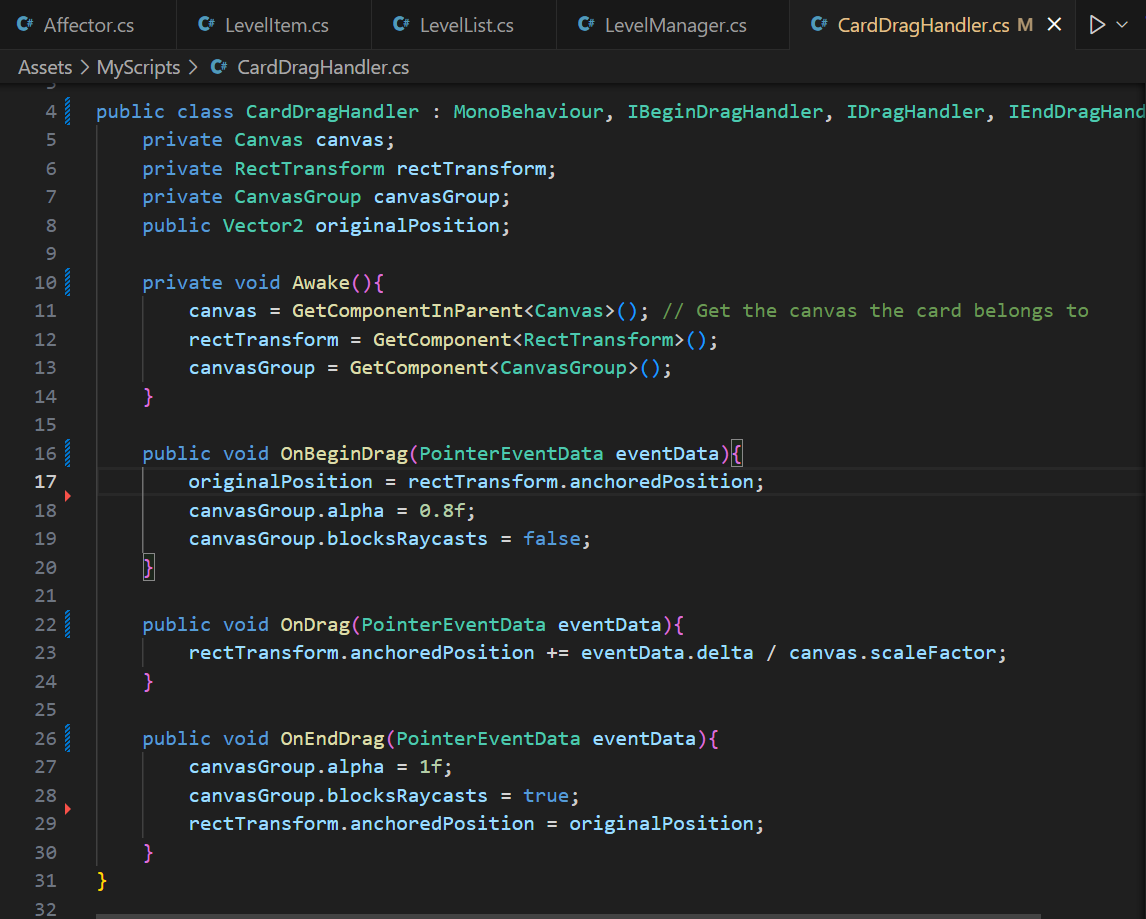
\includegraphics[scale=0.75]{images/CardDragHandler.png}
	\caption{CardDragHandler Script }
	\label{fig:CardDragHandler}
\end{figure}

\section{DropZone.cs}
\begin{figure}[h!]
	\centering
	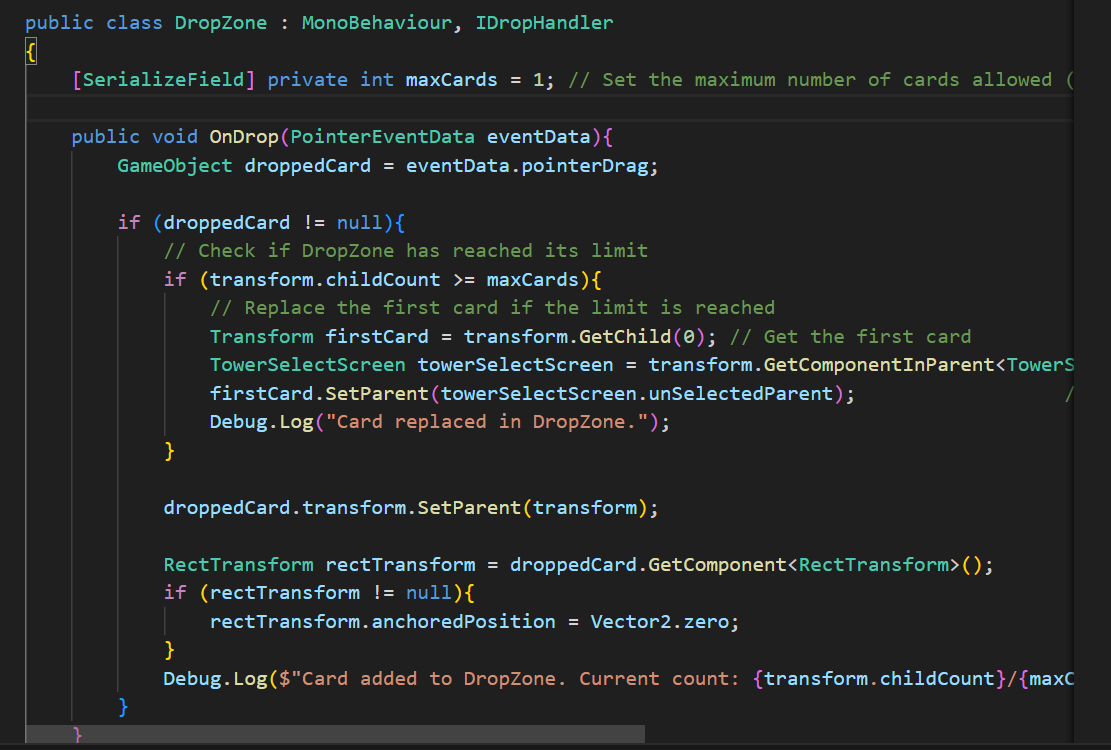
\includegraphics[scale=0.75]{images/DropZone.png}
	\caption{DropZone Script }
	\label{fig:DropZone}
\end{figure}

\section{TowerSelector.cs}
\begin{figure}[h!]
	\centering
	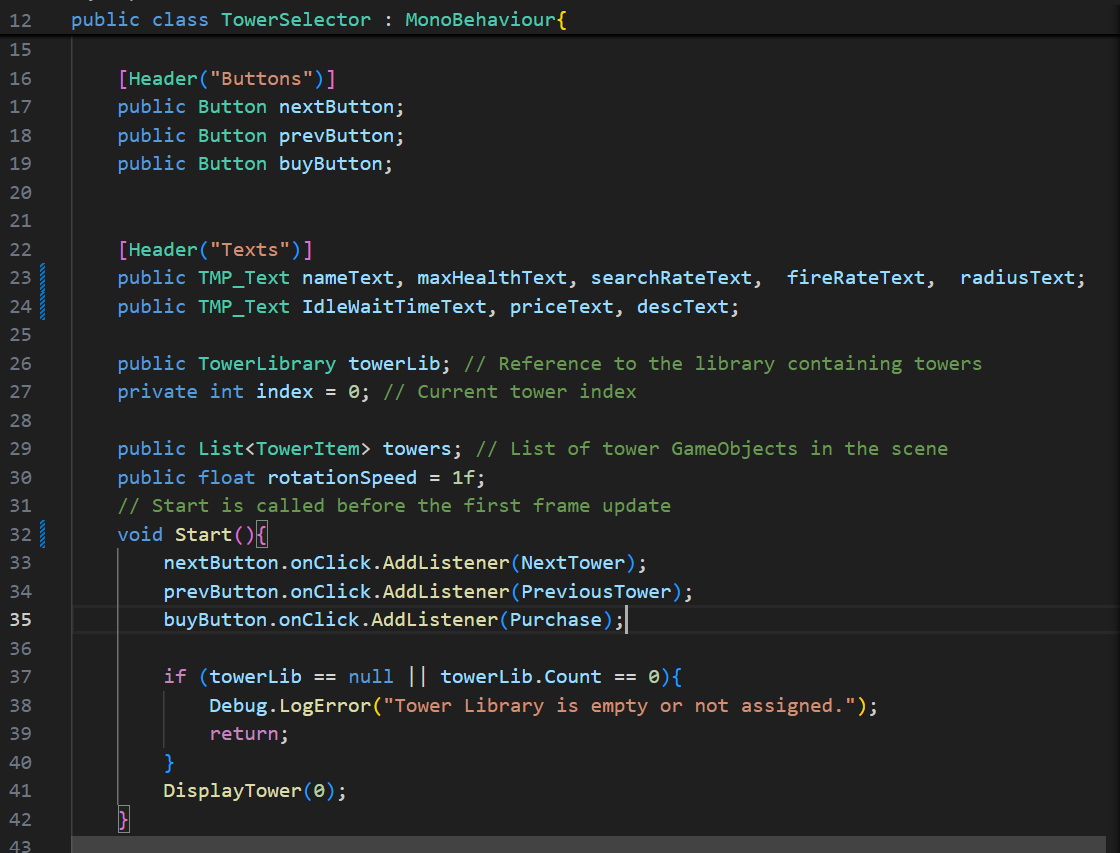
\includegraphics[scale=0.75]{images/TowerSelector1.png}
	\caption{TowerSelector Script Part 1}
	\label{fig:TowerSelector1}
\end{figure}

\begin{figure}[h!]
	\centering
	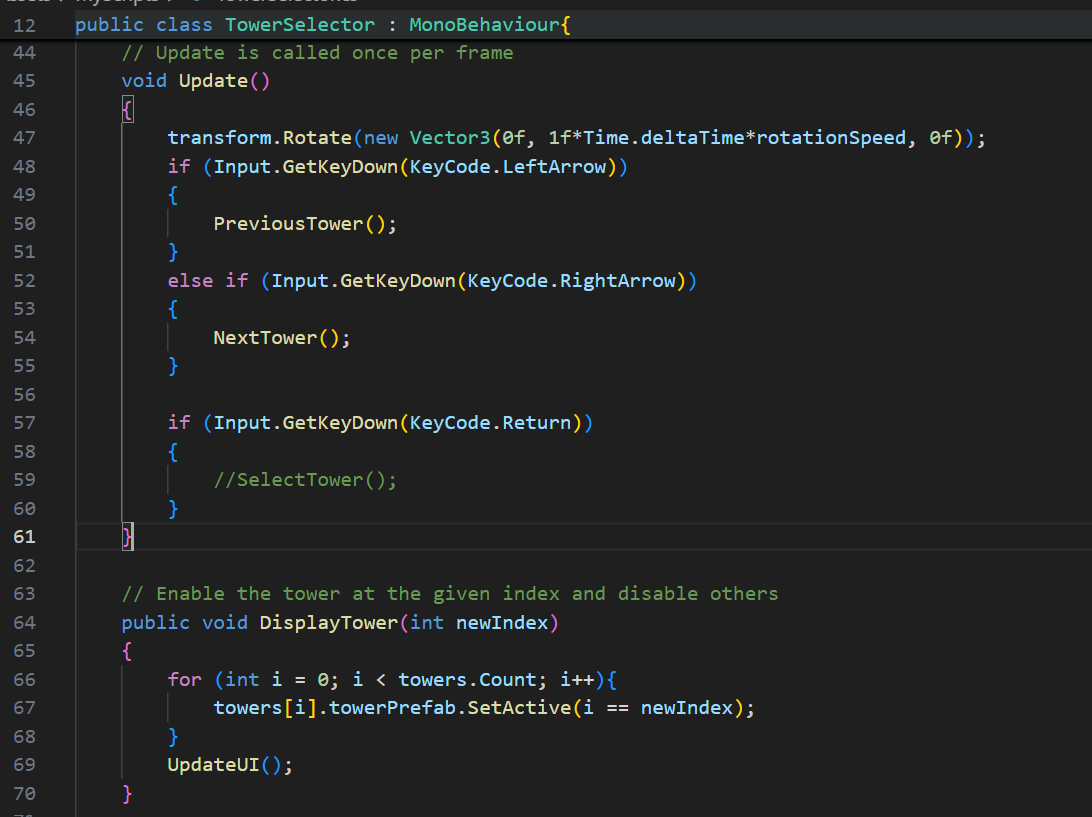
\includegraphics[scale=0.75]{images/TowerSelector2.png}
	\caption{TowerSelector Script Part 2}
	\label{fig:TowerSelector2}
\end{figure}

\begin{figure}[h!]
	\centering
	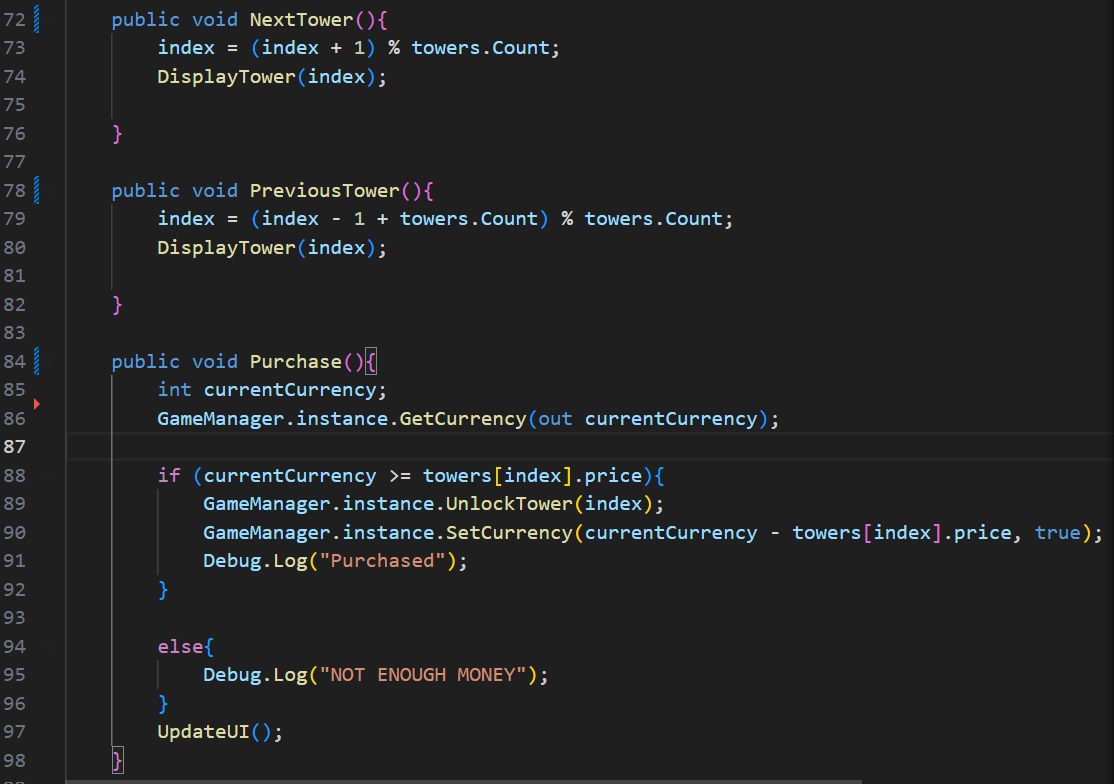
\includegraphics[scale=0.75]{images/TowerSelector3.png}
	\caption{TowerSelector Script Part 3}
	\label{fig:TowerSelector3}
\end{figure}

\begin{figure}[h!]
	\centering
	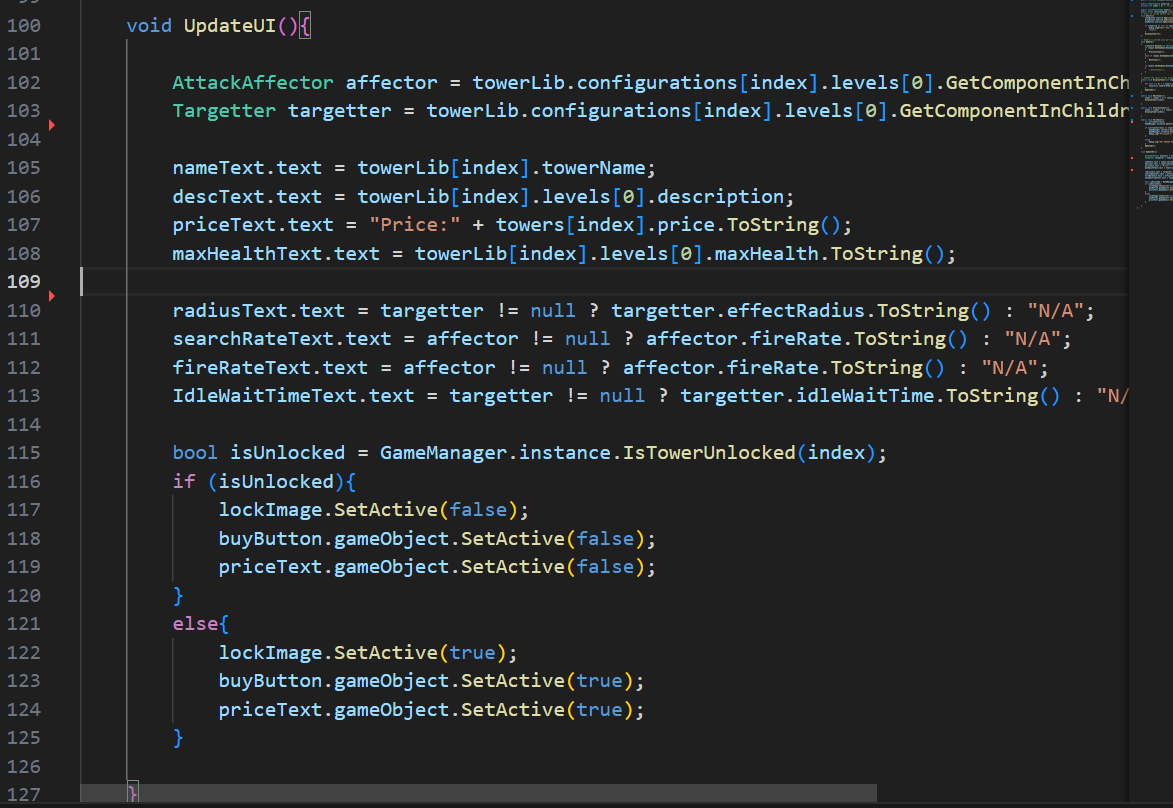
\includegraphics[scale=0.75]{images/TowerSelector4.png}
	\caption{TowerSelector Script Part 4}
	\label{fig:TowerSelector4}
\end{figure}


\chapter{Game Outputs}
\section{Menu and UIs} 

\begin{figure}[h!]
	\centering
	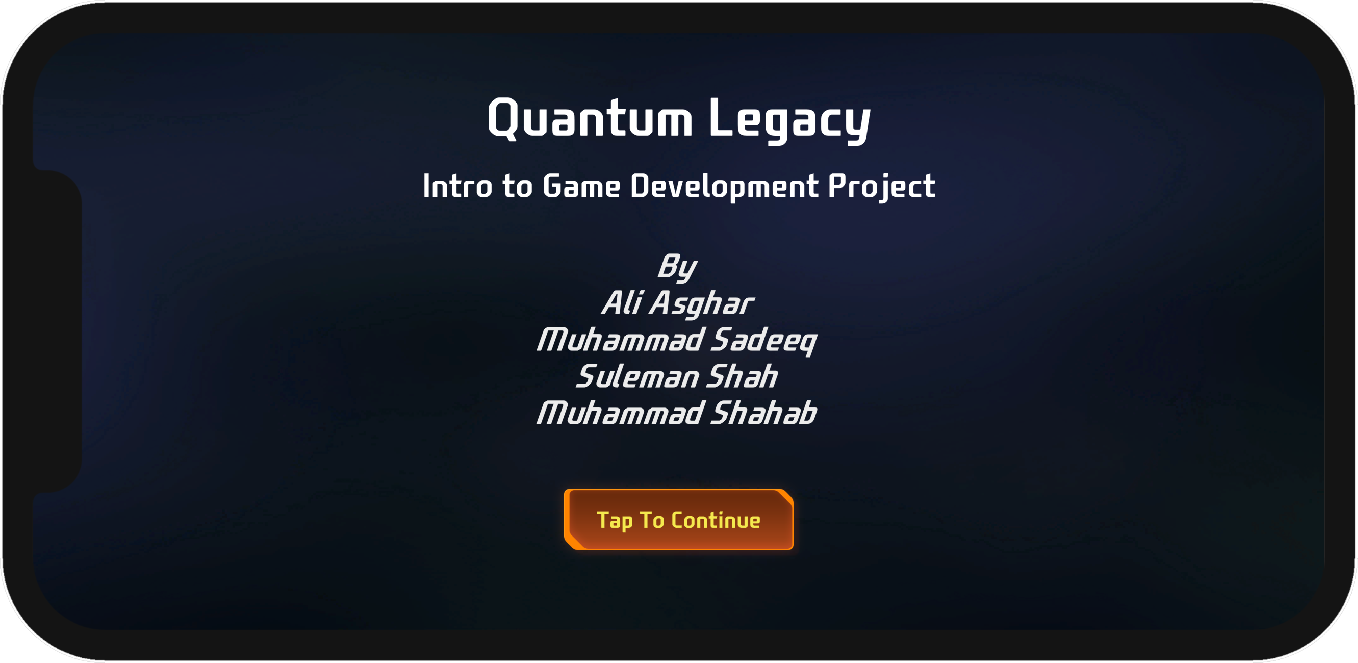
\includegraphics[scale=0.5]{images/SplashScreen.png}
	\caption{Splash Screen}
	\label{fig:SplashScreen}
\end{figure}

\begin{figure}[h!]
	\centering
	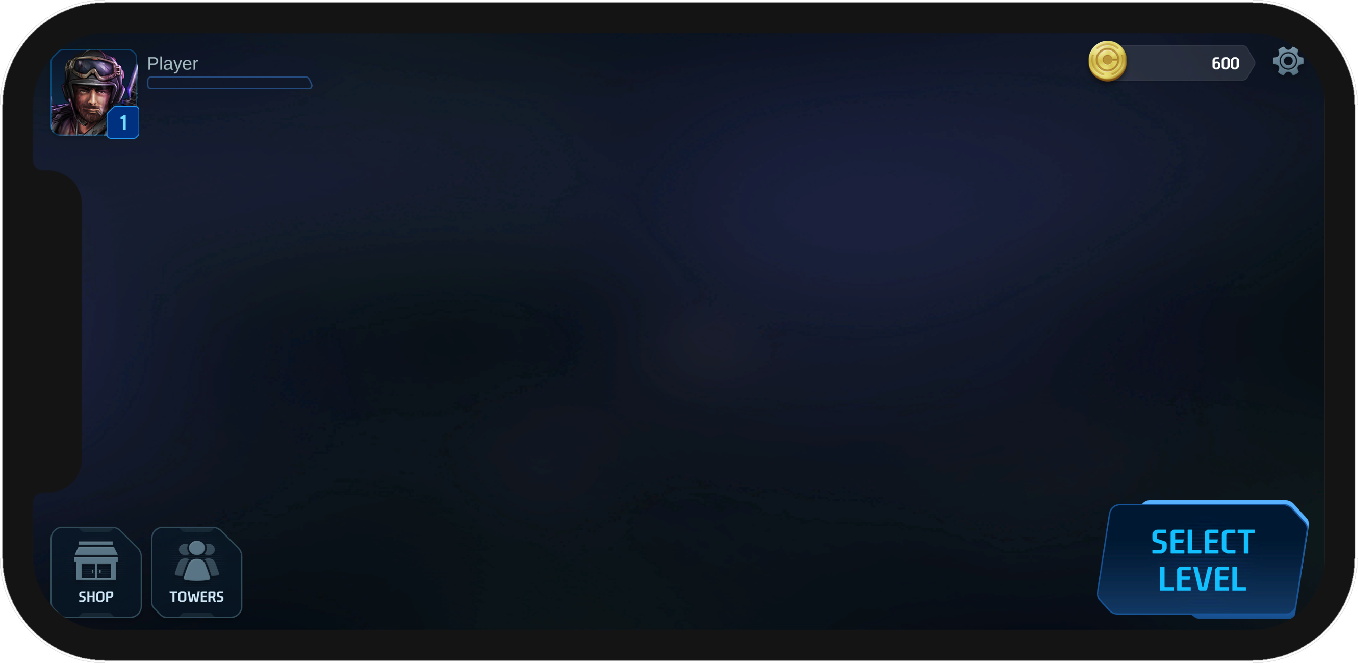
\includegraphics[scale=0.5]{images/MainMenuScreen.png}
	\caption{Main Menu Screen}
	\label{fig:MainMenuScreen}
\end{figure}

\begin{figure}[h!]
	\centering
	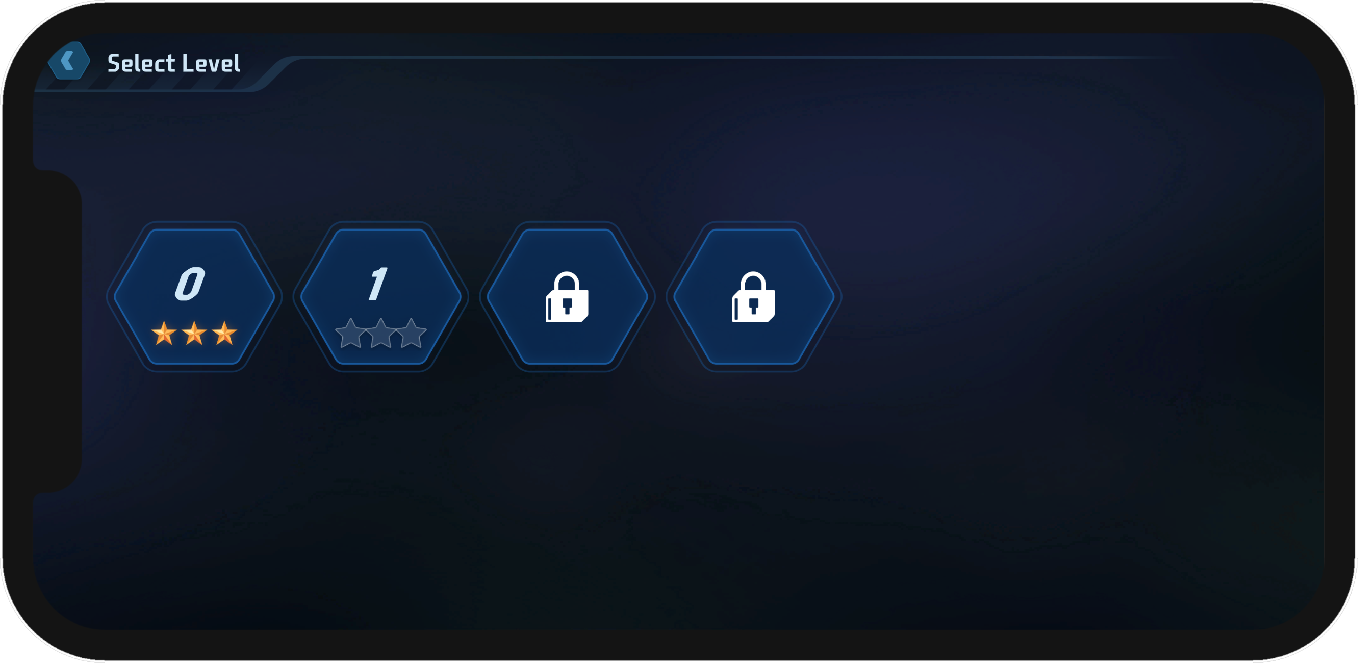
\includegraphics[scale=0.5]{images/LevelSelectScreen.png}
	\caption{Level Select Screen}
	\label{fig:LevelSelectScreen}
\end{figure}

\begin{figure}[h!]
	\centering
	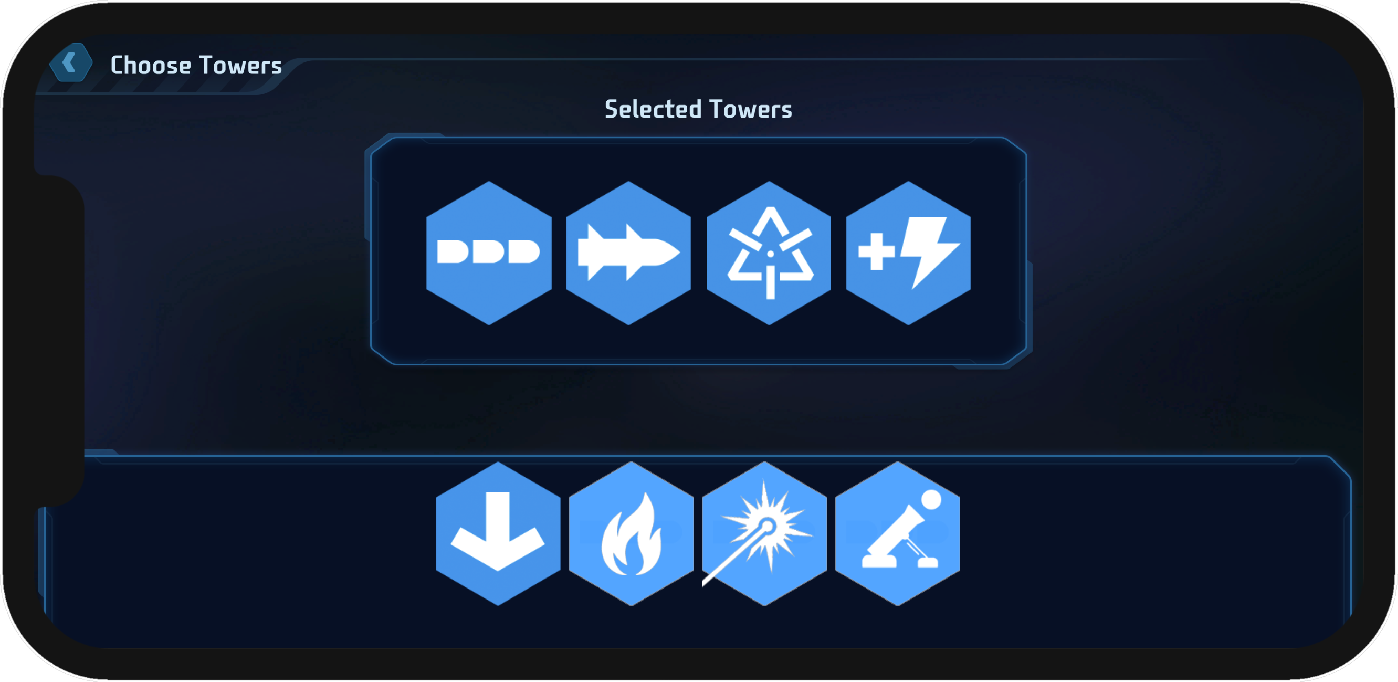
\includegraphics[scale=0.5]{images/SelectTowerScreen.png}
	\caption{Select Tower Screen}
	\label{fig:SelectTowerScreen}
\end{figure}

\begin{figure}[h!]
	\centering
	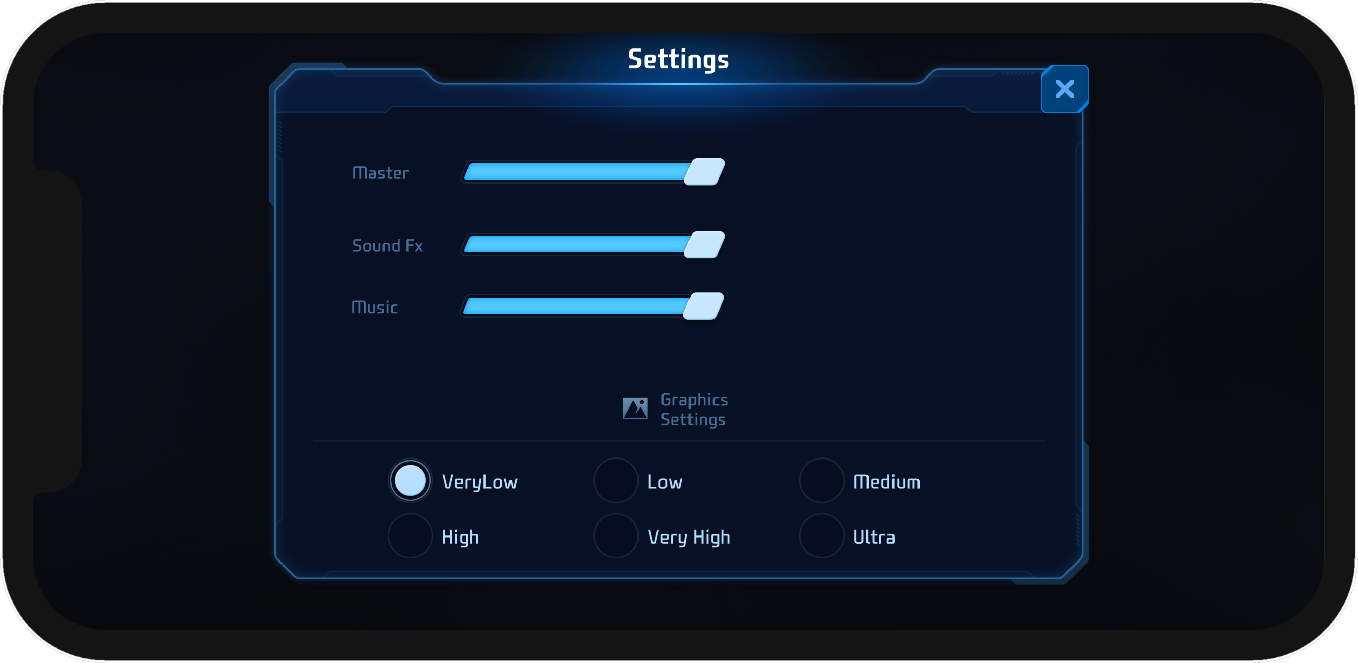
\includegraphics[scale=0.5]{images/SettingScreen.png}
	\caption{Settings Screen}
	\label{fig:SettingScreen}
\end{figure}

\begin{figure}[h!]
	\centering
	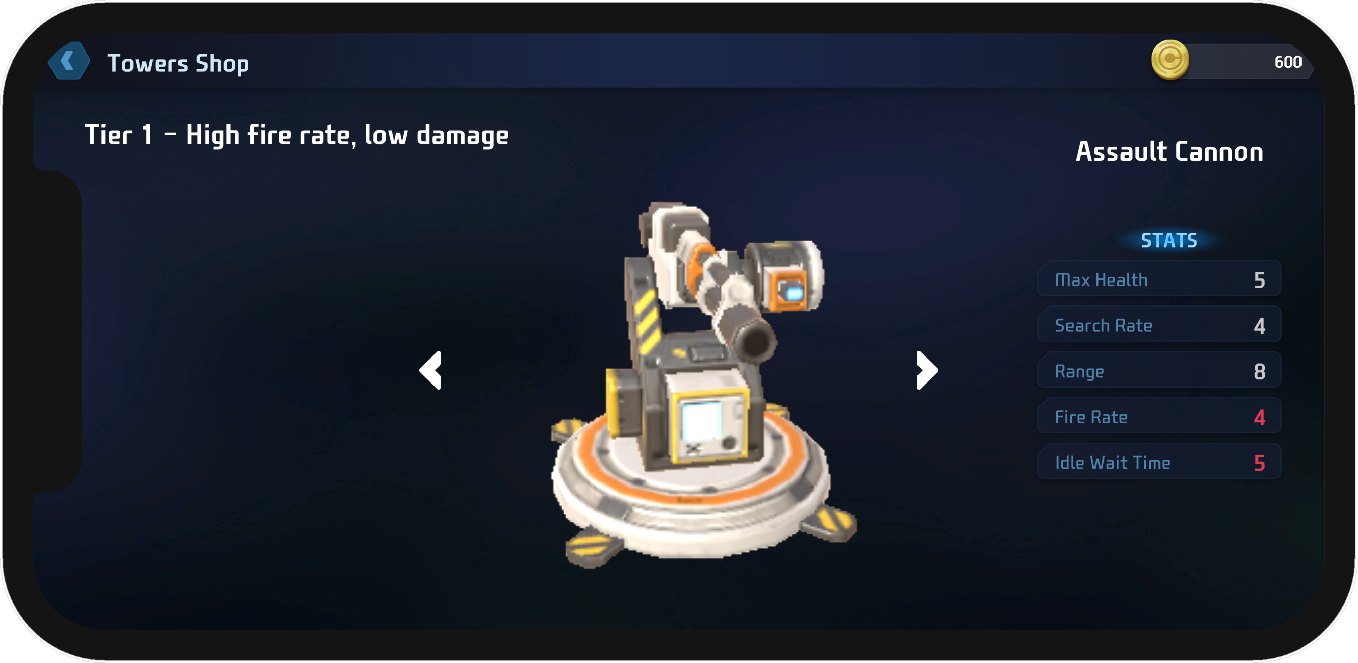
\includegraphics[scale=0.5]{images/TowerShopScreen.png}
	\caption{Tower Shop Screen}
	\label{fig:TowerShopScreen}
\end{figure}

\section{Gameplay} 

\begin{figure}[h!]
	\centering
	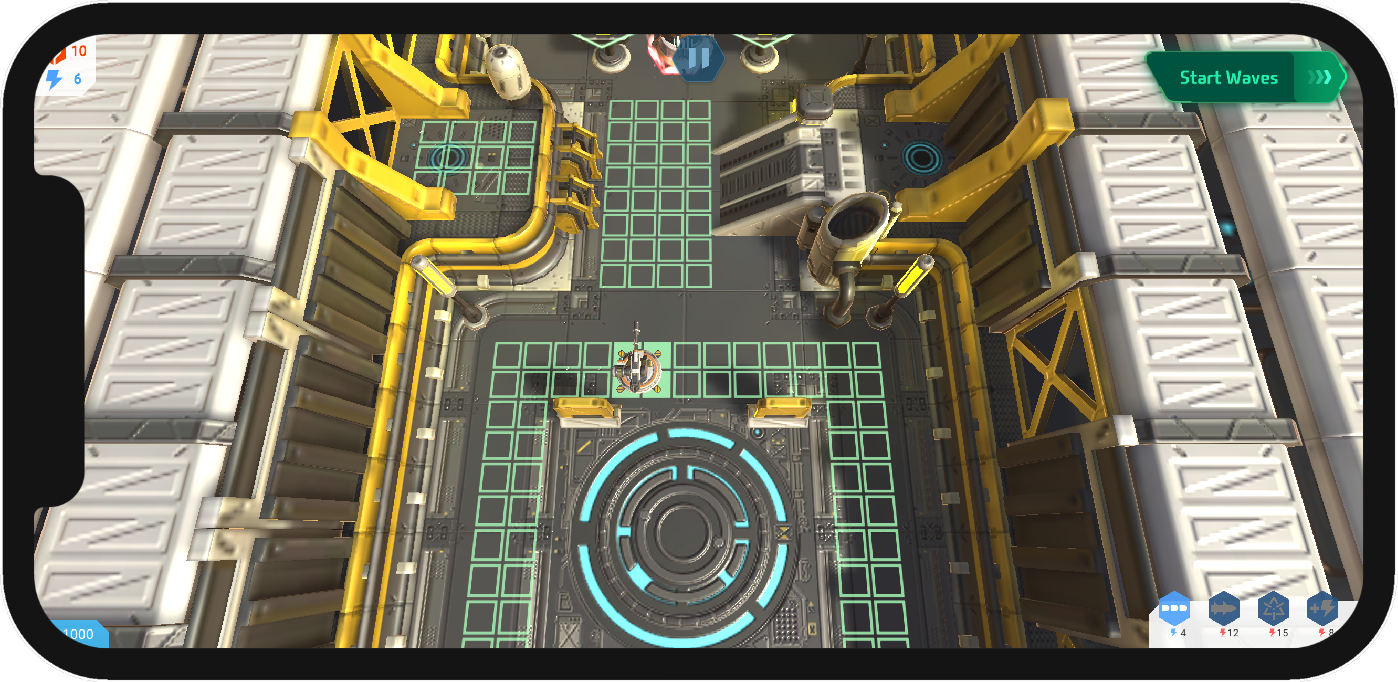
\includegraphics[scale=0.5]{images/Gameplay1.png}
	\caption{Gameplay Screenshot 1}
	\label{fig:Gameplay1}
\end{figure}

\begin{figure}[h!]
	\centering
	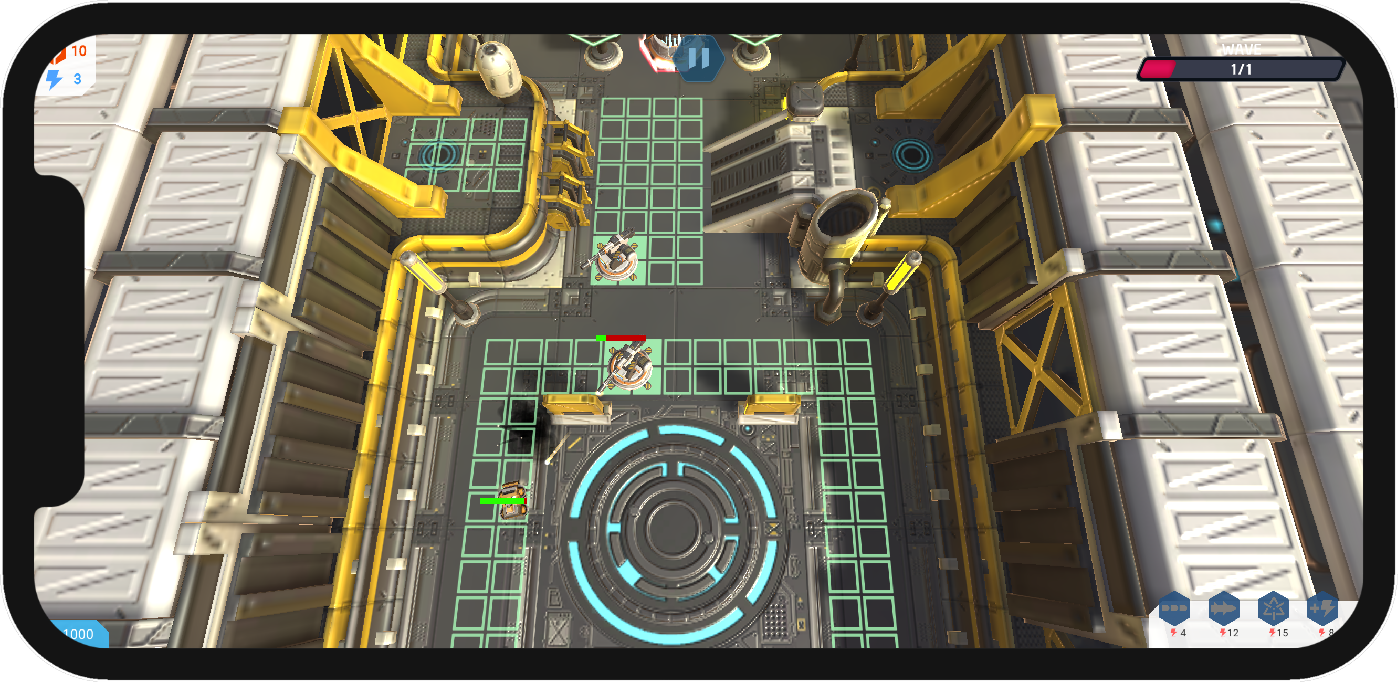
\includegraphics[scale=0.5]{images/Gameplay2.png}
	\caption{Gameplay Screenshot 2}
	\label{fig:Gameplay2}
\end{figure}




\chapter{Technical Specifications}
\section{General Info} 
\begin{itemize}
	\item \textbf{Engine:} Unity 
	\item \textbf{Art Style:} Futuristic, sci-fi aesthetic with vibrant colors and sleek designs.  
	\item \textbf{Audio:} Immersive sound effects and an original soundtrack to enhance the sci-fi atmosphere. 
	\item \textbf{Platforms:} PC (Windows, macOS), Mobile (iOS, Android). 
\end{itemize}

\section{Topics Covered from subject} 
\begin{itemize}
	\item C\# Classes
	\item GameObject Instantiation 
	\item Built-In Methods Like Update, Start, Awake etc
	\item Level Desig
\end{itemize}

\section{Role of Each Member} 

\begin{itemize}
	\item \textbf{Ali Asghar:} Main Lead Developer, responsible for designing the logic and game architecture.
	\item \textbf{Muhammad Sadeeq:} Co-Lead Developer, responsible for 3D environment and level designer.  
	\item \textbf{Suleman Shah:} Level Designer, responsible for testing and making levels interesting.
	\item \textbf{Muhammad Shahab:} UI Designer, responsible for making interactive and eye-catching UI.
\end{itemize}

\chapter{Conclusion}
This chapter gives the ending remarks and future work for our project.

\section{Future Updates}
\begin{itemize}
	\item \textbf{Multiplayer Mode:} Co-op or competitive tower defense. 
	\item \textbf{New Levels and Towers:} Expand the game with additional content.  
	\item \textbf{Story Mode:} Introduce a narrative-driven campaign. 
\end{itemize}
 
\section{Final Remarks}
Quantum Legacy is a visually stunning and strategically engaging tower defense game that combines sci-fi elements with addictive gameplay. With its unique towers, challenging levels, and robust progression system, it promises to captivate players and stand out in the tower defense genre.  
  
\end{document} 